\documentclass[12pt,a4paper]{article}
\usepackage{ctex}
\usepackage{amsmath,amscd,amsbsy,amssymb,latexsym,url,bm,amsthm}
\usepackage{epsfig,graphicx,subfigure}
\usepackage{enumitem,balance}
\usepackage{wrapfig}
\usepackage{mathrsfs,euscript}
\usepackage[usenames]{xcolor}
\usepackage{hyperref}
\usepackage[vlined,ruled,linesnumbered]{algorithm2e}
\usepackage{array}
\hypersetup{colorlinks=true,linkcolor=black}

\newtheorem{theorem}{Theorem}
\newtheorem{lemma}[theorem]{Lemma}
\newtheorem{proposition}[theorem]{Proposition}
\newtheorem{corollary}[theorem]{Corollary}
\newtheorem{exercise}{Exercise}
\newtheorem*{solution}{Solution}
\newtheorem{definition}{Definition}
\theoremstyle{definition}

\renewcommand{\thefootnote}{\fnsymbol{footnote}}

\newcommand{\postscript}[2]
 {\setlength{\epsfxsize}{#2\hsize}
  \centerline{\epsfbox{#1}}}

\renewcommand{\baselinestretch}{1.0}

\setlength{\oddsidemargin}{-0.365in}
\setlength{\evensidemargin}{-0.365in}
\setlength{\topmargin}{-0.3in}
\setlength{\headheight}{0in}
\setlength{\headsep}{0in}
\setlength{\textheight}{10.1in}
\setlength{\textwidth}{7in}
\makeatletter \renewenvironment{proof}[1][Proof] {\par\pushQED{\qed}\normalfont\topsep6\p@\@plus6\p@\relax\trivlist\item[\hskip\labelsep\bfseries#1\@addpunct{.}]\ignorespaces}{\popQED\endtrivlist\@endpefalse} \makeatother
\makeatletter
\renewenvironment{solution}[1][Solution] {\par\pushQED{\qed}\normalfont\topsep6\p@\@plus6\p@\relax\trivlist\item[\hskip\labelsep\bfseries#1\@addpunct{.}]\ignorespaces}{\popQED\endtrivlist\@endpefalse} \makeatother

\begin{document}
\noindent

%========================================================================
\noindent\framebox[\linewidth]{\shortstack[c]{
\Large{\textbf{Lab08-Graph Exploration}}\vspace{1mm}\\
CS214-Algorithm and Complexity, Xiaofeng Gao \& Lei Wang, Spring 2021.}}
\begin{center}
\footnotesize{\color{red}$*$ If there is any problem, please contact TA Yihao Xie. }

\footnotesize{\color{blue}$*$ Name:RenyangGuan  \quad Student ID:519021911058 \quad Email: guanrenyang@sjtu.edu.cn}
\end{center}

\begin{enumerate}

	\item Given an undirected graph $G = (V, E)$. Prove the following propositions.
	
	\begin{enumerate}
		\item Let $e$ be a maximum-weight edge on some cycle of connected graph $G=(V,E)$.
        Then there is a minimum spanning tree of $G$ that does not include $e$. Moreover, there is no minimum spanning tree of $G$ that includes $e$ if $e$ is the unique maximum-weight edge on the cycle. 
		\item Let $T$ and $T'$ are two different minimum spanning trees of $G$. Then $T'$ can be obtained from $T$ by repeatly substitute one edge in $T\backslash T'$ by one edge in $T'\backslash T$ and meanwhile the result after each subsitution is still a minimum spanning tree.
	\end{enumerate}
	\begin{solution}
	\begin{enumerate}
	    \item [(a)] The process of proof should be divided into two parts. One is to prove \textit{there is a minimum spanning tree of $G$ that does not include $e$.} and the other is to prove \textit{there is no minimum spanning tree of $G$ that includes $e$ if $e$ is the unique maximum-weight edge on the cycle.}
	    \\
	    \begin{enumerate}
	        \item [(1)] Let the cycle containing edge $e$ be denoted as $\{e,e_1,e_2,\cdots,e_k\}$. The proof is done by \textbf{contradiction}. Suppose none of the minimum spanning tree contains edge $e$. For each particular minimum spinning tree $T_i$, there exists an edge $e_i\in \{e,e_1,e_2,\cdots,e_k\}-\{e \}$, where $w(e_i)\leq w(e)$. The operation which remove $e$ and insert $e_i$ will reduce the total weight of the tree, which is a contradiction. 
	        \item [(2)] Let the two vertexes connected by $e$ are $v_i$ and $v_j$. The proof is also done by \textbf{contradiction}. Suppose that there is one minimum spinning tree $T_i$ containing edge $e$. The operation of deleting $e$ will divide the tree into two strong connected components, which are denoted as $SCC_i,SCC_j$ containing $v_i$ and $V_j$ respectively. Since there must be another edge $e'$ which connects $SCC_i$ and $SCC_j$ (otherwise the degree of $v_i$ or $v_j$ is $1$), adding $e'$ into the graph will connect the two strong connected components without adding cycle, which will reduce the total weight of $T_i$. This is a contradiction of the property of minimum spinning tree.
	    \end{enumerate}
	   
	   \item [(b)] The proof is done by \textbf{contradiction}. 
	   \\
	   Suppose that one particular operation makes $T''$ not a minimum spinning tree, which substitutes $e$ in $T\backslash T'$ by $e'$ in $T'\backslash T$ and generate $T''$. It means $w(e')<w(e)$. After deleting $e$, $T$ is divided into two strong connected components $SCC_i$ and $SCC_j$ and both of them are still trees. As a result, $e$ and $e'$ are involved in the same cycle in the raw graph, otherwise $SCC_i$ or $SCC_j$ will be connected by $e$ or $e'$ in $T$. 
	   \\
	   According to the conclusion in the previous question, the total weight of $T$ will be reduced if $e$ is substituted by $e'$. so $T$ is actually not a minimum spinning tree. This is a contradiction.
	  
	    
	\end{enumerate}
	\end{solution}
	    \item Let $G=(V,E)$ be a connected, undirected graph. Give an $O(|V|+|E|)$-time algorithm
    to compute a path in $G$ that traverses each edge in $E$ exactly once in each direction. Describe how you can find your way out of a maze if you are given enough coins to apply your algorighm.
    \begin{solution}
    Assuming that some vertices in $V$ is reachable while the others are not, the connected and undirected graph $G=(V,E)$ could denote the maze. Given a starting vertex and a finishing vertex, the algorithm is shown below 
    \\
        \begin{algorithm}[H]
		\KwIn{A graph $G=(V,E)$, starting vertex $v$, an array $V'$ initially set to $\emptyset$}
		\KwOut{A path of vertices $V'$}
		
		\BlankLine
		\caption{$EXPLORE(G,v,V')$}\label{Alg-maze}

        $V'\leftarrow V'\cup \{v\}$\;
        \BlankLine
		\If{$v$ is $v_{finish}$}
		{
		    \Return{$V'$}
		}
		\BlankLine
		\For{$\forall\ edge(u,v) \ \in \ E$}
		{
		    \If{$u\ \notin \ V'$ and $u$ is reachable}
		    {
		       $EXPLORE(G,u,V')$\;
		       $V'\leftarrow V'\cup \{v\}$\;
	    	}
		}
		\end{algorithm}
		
		\textbf{\textit{Time complexity analysis:}} 
		\\
		Over the course of the algorithm, each node will be explored at most once and each edge will be traversed at most twice. 
		\\
		As for the vertexes, if the point is not on the path, it will be added $V'$ at the end of the deeper recursion to represent that the traveler needs to pass through the node again when he returns.
		\\
		As for the edges, each edge is explored at most twice. Once is when it is firstly explored and the other is when the edge is not on the path from $v_{start}$ to $v_{finish}$. 
		\\
		As a result, the time complexity is 
		$$Time\ complexity=\ O(|V|+2|E|)=O(|V|+|E|)$$

	
    \end{solution}
    \item Consider the maze shown in Figure \ref{Fig-Maze}. The black blocks in the figure are blocks that can not be passed through. Suppose the block are explored in the order of right, down, left and up. That is, to go to the next block from $(X,Y)$, we always explore $(X,Y+1)$ first, and then $(X+1,Y)$,$(X,Y-1)$ and$(X-1,Y)$ at last. Answer the following subquestions:
    \begin{enumerate}
        \item Give the sequence of the blocks explored by using DFS to find a path from the "start" to the "finish".
        \item Give the sequence of the blocks explored by using BFS to find the \underline{shortest} path from the "start" to the "finish".
        \item Consider a maze with a larger size. Discuss which of BFS and DFS will be used to find one path and which will be used to find the shortest path from the start block to the finish block.
    \end{enumerate}
    
    
    \begin{figure}[!htbp]
	\centering
	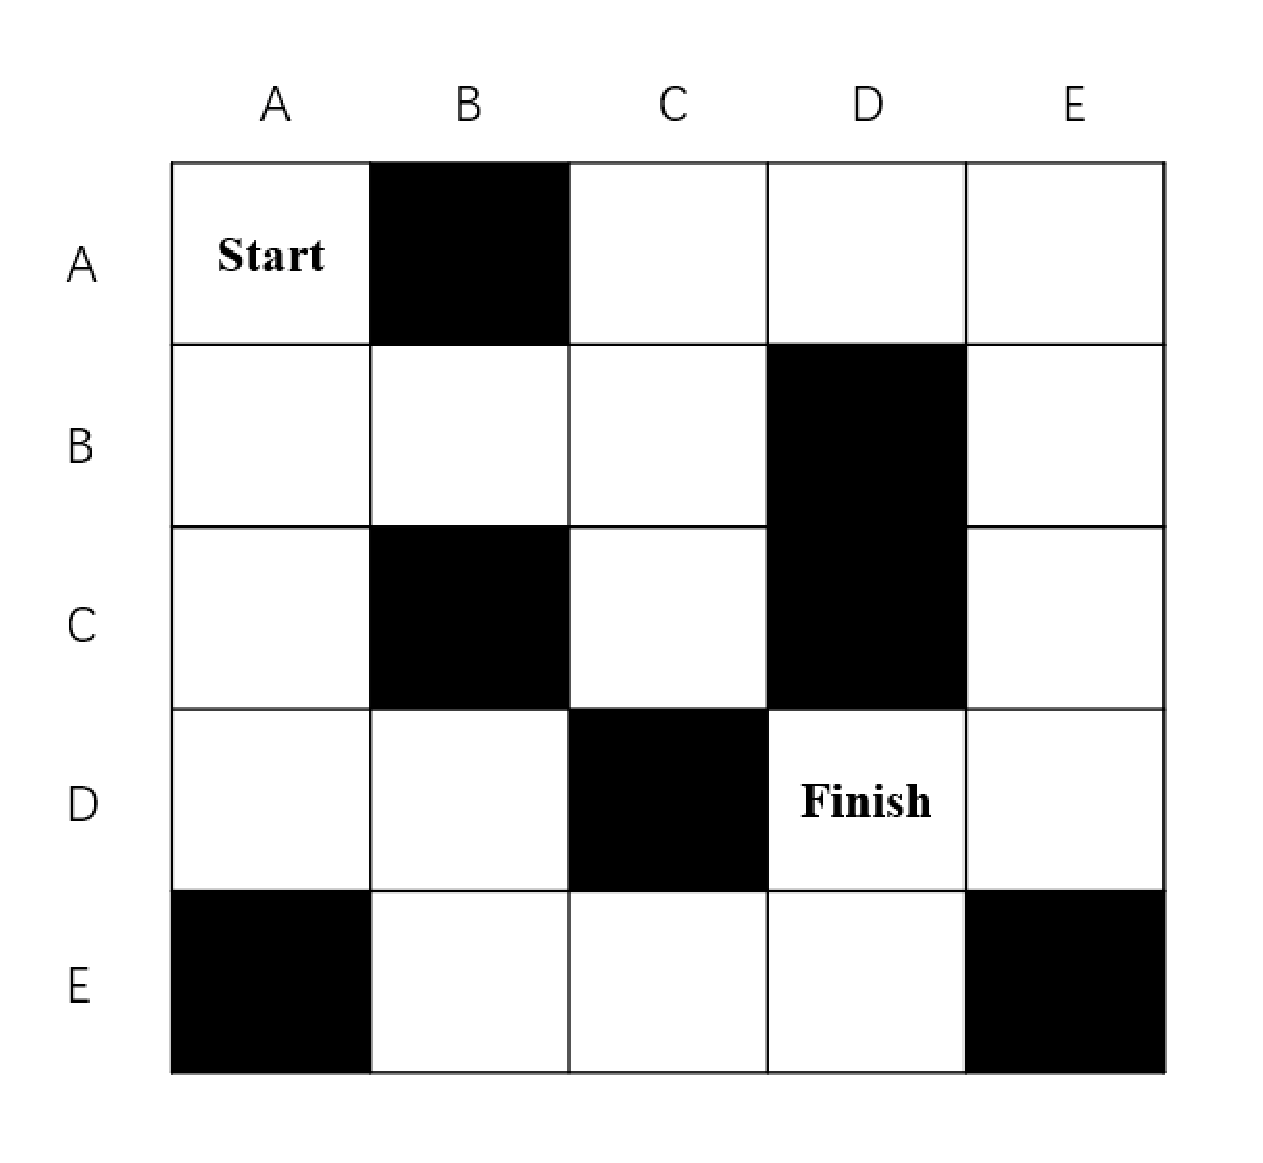
\includegraphics[width=0.45\textwidth]{Fig-Maze.pdf}
	\caption{The blocks in the maze.}
	\label{Fig-Maze}
	\end{figure}
	\begin{solution}
	~\\
	\begin{enumerate}
	    \item [(a)]
	    The sequence of blocks explored by DFS is 
	    $$(A,A),(B,A),(B,B),(B,C),(C,C),(A,C),(A,D),(A,E),(B,E),(C,E),(D,E),(D,D)$$
	    while the path is
	    $$(A,A),(B,A),(B,B),(B,C),(A,C),(A,D),(A,E),(B,E),(C,E),(D,E),(D,D)$$
	    \item [(b)]
	    The sequence of blocks explored by DFS is
	    $$(A,A),(B,A),(B,B),(C,A),(B,C),(D,A),(C,C),(D,B),(A,D),(E,B),(A,E),(E,C),(B,E),(E,D),(C,E),(D,D)$$
	    while the shortest path is
	    $$(A,A),(B,A),(C,A),(D,A),(D,B),(E,B),(E,C),(E,D),(D,D)$$
	    \item [(c)]
	    \textbf{BFS is more suitable for searching the shortest path}. DFS needs to traverse every possible path from start to end while BFS doesn't. Although BFS searches almost every node in the graph, there must be some node left.
	    \\
	    \textbf{DFS is more suitable for searching an existing path.} When the maze is of a huge size, there is a high possibility that the path exist in the former half of the maze and all the paths are of the similar length. As a result, the DFS will only traverse three forth of the vertices while the BFS will traverse all the vertices.
	\end{enumerate}
	\end{solution}
	\item Given a directed graph $G$, whose vertices and edges information are introduced in data file "SCC.in". Please find its number of Strongly Connected Components with respect to the following subquestions.
    
    \begin{enumerate}
    	\item Read the code and explanations of the provided C/C++ source code "SCC.cpp", and try to complete this implementation.
    	\item Visualize the above selected Strongly Connected Components for this graph $G$. Use the $Gephi$ or other software you preferred to draw the graph. {\color{blue}(If you feel that the data provided in ``SCC.in'' is not beautiful, you can also generate your own data with more vertices and edges than $G$ and draw an additional graph. Notice that results of your visualization will be taken into the consideration of Best Lab.)}
    \end{enumerate}	
    \begin{figure}[!htbp]
	\centering
	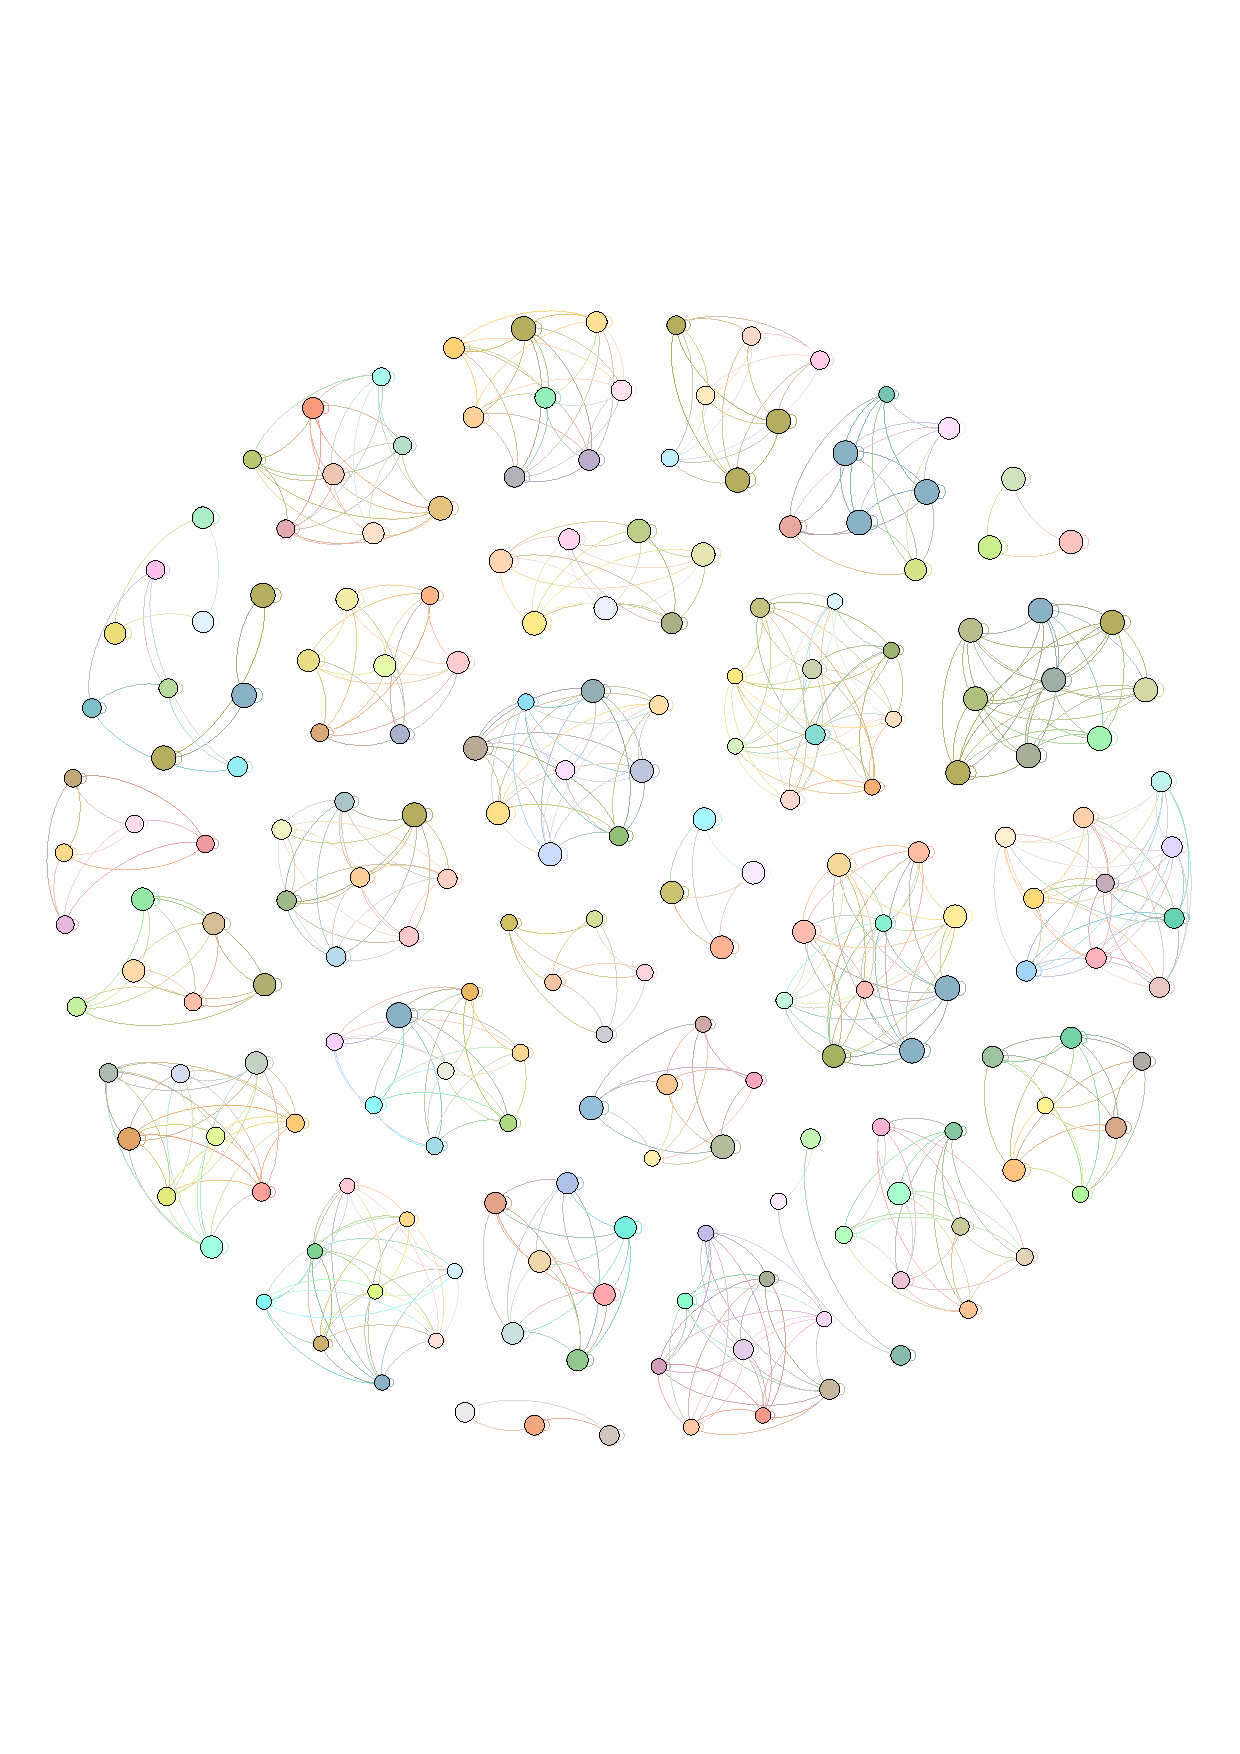
\includegraphics[width=0.8\textwidth]{Fig-SCC.pdf}
	\caption{The graph of strong connected components.}
	\label{Fig-SCC}
	\end{figure}
    \begin{solution}
    The graph of strong connected components is shown in Fig.~\ref{Fig-SCC}. It merges all the node belonging to the same strong connected component in a node and uses the size of node to denotes the number of nodes the strong connected component containing.
    
    \end{solution}
\end{enumerate}



\textbf{Remark:} Please include your .pdf, .tex, .cpp files for uploading with standard file names.
\newpage


%========================================================================
\end{document}